%  Autor: Michael Entrup geb. Epping
%  E-Mail: michael.entrup@wwu.de
%  Version: 1.7.2
%  Datum: April 2016
%  Info: Dies is eine komplexe Vorlage für das erstellen einer Abschlussarbeit.
%		Um den Inhalt von sonstigen Dingen zu trennen, besteht die Vorlage aus mehreren Dateien.
%		Dies ist die Hauptdatei. Sie sollte nicht verändert werden.
%		Hier werden die Einstellungen festgelegt und Pakete eingebunden.
%		Alles weitere wird über die Dateien verändert, die mit "0X_" beginnen.
%		Für den eigentliche Inhalt sollten folglich die Dateien "10_Inhalt.tex" und "20_Anhang.tex" verwendet werden.
%  Copyright: CC BY 4.0 (http://creativecommons.org/licenses/by/4.0/)

% Änderungen 1.2 -> 1.3
% * Bei der Verwendung von texlive2012 gibt es Probleme mit myalphadin.
%   Diese Vorlage für Einträge insLiteraturverzeichnis habe ich durch unsrtdin ersetzt.
% * Da ich jetzt mit TeXlipse arbeite, habe ich ein paar Anpassungen vorgenommen.
%   So ist z.B. der Name der bib-Datei fest vorgegeben, damit auch die Autovervollständigung bei BibTeX-Keys funktioniert.
% * Zusätzliche Kommentare sollten das Arbeiten mit dieser Vorlage erleichtern.
% * Die Vorlage enthält sinnvollen Text und nicht nur nutzlose Platzhalter.

% Änderungen 1.3 -> 1.4
% * Das Paket "ifthenx" gibt es unter Ubuntu 12.04 mit texlive 2009-15 nicht. Als alternative habe ich "xifthen" eingetragen.
% * Tabulatoren habe ich durch Leerzeichen ersetzt. Dadurch bleibt das Layout (Einrücken und Position Kommentare) erhalten,
%   egal mit welchem Editor man die Dateien öffnet.
% * Ich habe einen Copyright-Vermerk hinzugefügt, nämlich dass es im Prizip keines gibt.
% * Neuer Abschnitt: latexmk
% * Neuer Abschnitt: Verbatim
% * Die Bilddatei "titelseite.jpg" wurde entfernt (wegen Copyright), da die Vorlage ab jetzt öffentlich zugänglich sein soll.
% * "README.txt" im Verzeichnis Bilder wurde erstellt.
% * Literaturangabe der Anleitung zur Optik, Wärmelehre und Atomphysik hinzugefügt.

% Änderungen 1.4 -> 1.5
% * Meinen Namen und meine E-Mail geändert.
% * Info zur Angabe einer E-Mail Adresse hinzugefügt.

% Änderungen 1.5 -> 1.6
% * Kapitel zum Einrichten von Texmaker hinzugefügt.

% Änderungen 1.6 -> 1.6.1
% * \usepackage{microtype} hinzugefügt.
% * \usepackage[T1]{fontenc} musste ich entfernen, da es nicht kompatibel zu microtype ist.
% * Ich habe die Links zu den Paketdokumentationen (Anhang) aktualisiert.
% * Ich habe die Pakete 'subfig' und 'warpfig' entfernt, da sie nicht verwendet werden.

% Änderungen 1.6.1 -> 1.7.0
% * Zweck der Vorlage geändert:
%	* Diese Vorlage war ursprünglich für ein Protokoll gedacht, dafür ist sie jedoch zu komplex.
%	* Mit 1.7.0 wird die Vorlage für eine Abschlussarbeit angepasst.
%   * Titelseite an eine Abschlussarbeit angepasst.
% * Die Titelseite erhält ein neues Logo (https://www.iconfinder.com/icons/9098/file_latex_tex_icon#size=128).
% * Die Dokumentenklasse wurde in scrbook geändert und deshalb wurden Kapitel eingefügt.
% * Kopf- und Fußzeile überarbeitet:
%   * scrlayer-scrpage statt scrpage2
%   * Autor und Kapitel stehen in der Kopfzeile.
%   * Die Seitenzahl steht immer außen in der Fußzeile.
%   * Informationen zu scrheadings und plain.scrheadings wurden zu den Kommentaren hinzugefügt.

% Änderungen 1.7.0 -> 1.7.1
% * Inhalt der Anleitung überarbeitet:
%   * TeXstudio als favorisierten Editor hinzugefügt
%   * Grammatikkorrektur mit LanguageTool für Verbesserungen genutzt

% Änderungen 1.7.1 -> 1.7.2
% * Fehler bei zweiseitigem Layout behoben:
%   * Nach der Titelseite wurde keine Leerseite eingefügt. Ursache war das Umschalten auf römische Seitenzahl. Durch ein cleardoublepage lässt sich das Problem beheben.

% ###############
% # Allgemeines #
% ###############

% Zeilen, die mit einem Prozentzeichen beginnen sind Kommentare.
% Alle verwendeten Funktionen sind mit solchen Kommentaren versehen, so dass man den Zweck der jeweiligen Funktion nachvollziehen kann.

% ######################################
% # Konfigurieren der Dokumentenklasse #
% ######################################

\documentclass[
% Dies sind globale Parameter. Sie gelten für die Dokumentenklasse selbst, aber auch für Pakete, welche später geladen werden.
	% Papierformat
	paper=a4,
    % Zweiseitig oder Einseitig
    twoside=false,
    % BCOR steht für Bindekorrektur und fügt einen zusätzlichen Rand ein. Da man eine Abschlussarbeit für gewöhnlich bindet, sollte man diesen Wert an die verwendete Bindung anpassen.
    BCOR=0mm,
    % Schriftgröße
    fontsize=12pt,
	% schreibt die Papiergröße korrekt ins Ausgabedokument
    pagesize=auto,
    % Normalerweise wird die erste Zeile eines Absatzes eingerückt, um diesen hervorzuheben. Als Alternative kann man parskip aktivieren, womit statt dem Einrücken ein vertikaler Abstand verwendet wird. Mögliche Werte sind half und full.
    %parskip=half,
    % Linie unterhalb der Kopfzeile
    headsepline=true,
    % Kapitelnummern (in Kopfzeile), Bildunterschrift und Tabellenüberschriften erhalten keinen abschließenden Punkt. Alternative: enddot
    numbers=noenddot,
    % Markiert zu lange und zu kurze Zeilen. Die PDF-Datei enthält außerdem keine klickbarebn Links mehr.
    draft=false
]{scrbook}
% Es gibt die Dokumenttypen scrartcle, srcbook, scrreprt und scrlettr. Diese gehören zum KOMA-Skript und sollten für deutsche Texte benutzt werden.
% Für englische Texte wählt man entsprechend article, book, report und letter.
% Es ist  nicht unbedingt zu empfehlen, bei einem bestehendem Dokument, die documentclass zu ändern.

% ####################
% # Pakete einbinden #
% ####################

% Pakete erweitern LaTeX um zusätzliche Funktionen. Dies ist eine Satz nützlicher Pakete.
% Weitere sollten in der Datei"`01_EigenePakete.tex"' hinzugefügt werden.

% Legt die Zeichenkodierung fest, z.B UTF8
\usepackage[utf8]{inputenc}
% Silbentrennung nach neuer deutscher und englischer Rechtschreibung
\usepackage[ngerman,english]{babel}
% Mathepaket
\usepackage{amsmath}
% Wird benötigt um \ifthenelse zu benutzen
\usepackage{xifthen}
% Zum flexiblen Einbinden von Grafiken, pdftex ist optional
\usepackage[pdftex]{graphicx}
% Ermöglicht die Nutzung von \unit[Zahl]{Einheit}
\usepackage{units}
% Einfaches wechseln zwischen unterschiedlichen Zeilenabständen
\usepackage{setspace}
% Darstellung für Caption s.u.
\usepackage[font=small,labelfont=bf,labelsep=endash,format=plain]{caption}
% Zusatzfunktionen zum zitieren
\usepackage{cite}
% Wird für Kopf- und Fußzeile benötigt.
% Es gibt Alternativen, für Klassen aus dem KOMA-Script sollte scrlayer-scrpage verwendet werden.
\usepackage{scrlayer-scrpage}
% Beide Pakete werden für die Ausrichtung der Tabellenspalten benötigt.
\usepackage{array,dcolumn}
% Verlinkt Textstellen im PDF Dokument. Es wird empfohlen dieses Paket immer zuletzt zu laden.
\usepackage[pdfpagelabels]{hyperref}
% Abstände zwischen Buchstaben und Wörtern werden verbessert.
% Dies führt z.B. dazu, dass weniger Silbentrennung genutzt wird.
\usepackage{microtype}

% weitere Pakete einbinden
% Die Folgenden Pakete sind schon eingebunden (siehe 00_Protokoll.tex):
%\usepackage[utf8]{inputenc}
%\usepackage[ngerman,english]{babel}
%\usepackage{amsmath}
%\usepackage{xifthen}
%\usepackage[pdftex]{graphicx}
%\usepackage{units}
%\usepackage{setspace}
%\usepackage[font=small,labelfont=bf,labelsep=endash,format=plain]{caption}
%\usepackage{cite}
%\usepackage{scrlayer-scrpage}
%\usepackage{array,dcolumn}
%\usepackage[pdfpagelabels]{hyperref}
%\usepackage{microtype}


% ############################
% # Eigene Befehle einbinden #
% ############################

% Eigene Befehle eignen sich gut um Abkürzungen für lange Befehle zu erstellen. Die Syntax ist folgende:
% \newcommand{neuer Befahl}{ein langer Befehl}
% Das folgende Beispiel fügt ein Bild mit bestimmten vorgegebenen Optionen ein:
\newcommand{\cImage}[2][0.5]{
    \begin{figure}[h!]
        \centering
        \includegraphics[width=#1\textwidth]{#2}
    \end{figure}
}
% #1 und #2 sind Parameter, die man \cImage übergeben muss. In 10_Titelseite.tex wird dieser Befehl verwendet. Der Parameter ist dort Bilder/titelseite.jpg.
% Benötigt man keine Parameter, dann lässt man [2] weg. Werden zusätzliche Parameter benötigt, dann kann man die Zahl auf maximal 9 erhöhen.


% #########################
% # Variablen importieren #
% #########################

% Der Befehl \newcommand kann auch benutzt werden um Variablen zu definieren:

% Titel der Arbeit:
    \newcommand{\varTitel}{Vorlage für eine Abschlussarbeit}
% Datum der Abgabe:
    \newcommand{\varDate}{\today}
% Autoren der Arbeit:
    \newcommand{\varAutor}{Michael Entrup}
% Weitere angaben unterhalb des Autors:
	\newcommand{\varInfo}{Abschlussarbeit\\im Fachbereich Physik\\der WWU Münster}
% E-Mail-Adressen der Autoren:
% Enthält eure Adresse einen Unterstrich, so müsst ihr '\_' verwenden!
    \newcommand{\varEmail}{michael.entrup@wwu.de}
% E-Mail-Adresse anzeigen (true/false):
    \newcommand{\varZeigeEmail}{true}
% Literaturverzeichnis anzeigen (true/false):
    \newcommand{\varZeigeLiteraturverzeichnis}{true}
% Stil der Einträge im Literaturverzeichnis
    \newcommand{\varLiteraturLayout}{unsrtdin}

% Definiert die Variable 'show', die später noch verwendet wird.
\newboolean{show}

% #########################
% # Beginn des Dokumentes #
% #########################

\begin{document}
	% Schreibsprache Deutsch.
	\selectlanguage{ngerman}
	% 1 1/2 facher Zeilenabstand für bessere Lesbarkeit.
	\onehalfspacing
	% Überschriften erhalten Serifen.
	% Standart ist '\sffamily', also Serifenfrei. Alternativ ist auf '\ttfamily' möglich.
	\addtokomafont{sectioning}{\rmfamily}
	% Nummerierung der Formeln entsprechend der Section (z.B. 1.1).
	\numberwithin{equation}{section}
	% Ändert Schriftgröße und Zeilenabstand bei captions von Bildern und Tabellen.
	\addtokomafont{caption}{\small\linespread{1}\selectfont}

% #######################################
% # Kopf- und Fußzeile konfigurieren    #
% #######################################

	% In 05_Kopf-Fuß.tex kann man Kopf- und Fußzeile verändern.
	% Löscht man die Datei 05_Kopf-Fuß.tex, dann wird die Standardeinstellung verwendet.
	\IfFileExists{05_Kopf-Fuss}{
		% Die Kopf- und Fußzeile werden mit Hilfe des Paketes scrpage2 konfiguriert.
% Durch die Verwendung von Innen- und Außenseite eignet sich das Layout für ein- und doppelseitige Dokumente.

% Latex unterscheidet zwischen dem normalen Seitenstil und dem Stil plain.
% Letzterer wird für den Beginn von Kapiteln verwendet.
% In diesem Dokument heißen die Stile scrheadings und plain.scrheadings, da das Paket scrlayer-scrpage verwendet wird.
% LaTeX schaltet automatisch zwischen beiden um, wenn einer aktiviert wurde (mit \pagestyle{scrheadings}).

% Die folgenden Befehle benötigen deshalb 2 Parameter.
% Der optionale Parameter (in eckigen Klammern) ist für den Seitenstil plain.scrheadings gedacht.
% Der zweite Parameter (in geschweiften Klammern) ist für den Seitenstil scrheadings gedacht.
% Beginnt ein neues Kapitel, dann ist es nicht nötig, dass man das Kapitel erneut in die Kopfzeile schreibt.
% Auf allen anderen Seiten soll die Titelseite den Autor (Links) und das Kapitel (Rechts) enthalten.
% Die Fußzeile soll bei allen Seiten identisch sein.

% Innenseite der Kopfzeile
\ihead[]{\varAutor} 
% Mitte der Kopfzeile                     
\chead{}            
% Außenseite der Kopfzeile                                       
\ohead[]{\headmark}
	
% Innnenseite der Fußzeile									           
\ifoot[]{}   
% Mitte der Fußzeile                                                
\cfoot[]{}     
% Aussenseite der Fußzeile                        
\ofoot[\pagemark]{\pagemark}  

% Alternative, wie sie häufig bei Büchern verwendet wird:
%\ihead[]{}                   
%\chead{}                                                  
%\ohead[\pagemark]{\headmark\qquad\pagemark}       							           
%\ifoot[]{}                                                 
%\cfoot[]{}                            
%\ofoot[]{} 
	} % Nach \IfFileExists muss eine Leerzeile eingefügt werden

% ###################################
% # Ausrichtung der Tabellenspalten #
% ###################################

	% , in Tabellen untereinander stellen
	\newcolumntype{,}{D{,}{,}{-1}}
	% +- in Tabellen untereinander stellen
	\newcolumntype{p}{D{p}{\pm}{-1}}

% ########################
% # Titelseite einbinden #
% ########################

	\begin{titlepage}
    \vspace*{4cm}
    \begin{center}
        \Huge
        \textbf{\varTitel}\\
        \vspace{2,5cm}
        \IfFileExists{Bilder/titelseite.png}{
            \cImage{Bilder/titelseite.png}
        } % Nach \IfFileExists muss eine Leerzeile eingefügt werden

        \vspace{1,5cm}        
        \large
        \varAutor
        \normalsize
        \newboolean{showEmail}
        \setboolean{showEmail}{\varZeigeEmail}
        \ifthenelse{\boolean{showEmail}}{\\\textit{\varEmail}\\}{}
        \vspace{1,5cm}
        \large
        \varInfo \\
        \varDate
    \end{center}
\end{titlepage}


	% Römische Ziffern als Seitenzahlen für das Inhaltsverzeichnis
	% cleardoublepage ist notwendig, damit bei zweiseitigem Layout nach der Titelseite eine leere Seite eingefügt wird.
	\cleardoublepage
	\setcounter{page}{1}
	\pagenumbering{Roman}

% ################################
% # Inhaltsverzeichnis einbinden #
% ################################

	\tableofcontents
	\newpage

	% Zurücksetzen der Seitenzahlen auf arabische Ziffern
	\setcounter{page}{1}
	\pagenumbering{arabic}

	% Ab hier mit Kopf- und Fußzeile
	\pagestyle{scrheadings}

% ###################################
% # Den Inhalt der Arbeit einbinden #
% ###################################

	\chapter{Einleitung}

% Anmerkung: Steht \LaTeX einzeln im Text, dann muss es mit \ beendet werden. Nur so wird auch das folgende Leerzeichen berücksichtigt.
Diese Vorlage soll euch den Einstieg in \LaTeX\ erleichtern. Habt ihr schon eine \LaTeX-Distribution installiert und am besten einen \LaTeX-Editor mit Syntax-Hervorhebung und Autovervollständigung, könnt ihr direkt loslegen. Eine Übersicht vieler Editoren ist in Abschnitt \ref{sec:editoren} zu finden. Mein Favorit ist aktuell TeXstudio\footnote{\url{http://texstudio.sourceforge.net/}}. Am Anfang reicht es aus die Dateien \verb|03_Variablen.tex|, \verb|10_Inhalt.tex| und \verb|20_Anhang.tex|\footnote{Die Zahlen dienen dazu die Dateien zu sortieren. Ich habe außerdem keine fortlaufenden Zahlen verwendet, damit es einfach möglich ist weitere Dokumente zwischen die bestehenden einzufügen.} zu bearbeiten. Benötigt ihr keinen Anhang, löscht einfach die Datei \verb|20_Anhang.tex|.

Habt ihr euch erst mal etwas mit \LaTeX\ beschäftigt, so sollte ihr auch mal in die anderen Dateien schauen. Die vielen Kommentare helfen hoffentlich dabei zu verstehen, was die einzelnen Befehle bewirken. Die umfangreichen Dokumentationen zu den verwendeten Paketen sind im Anhang (\ref{anhang}) verlinkt.

Da ich an der WWU Münster Physik studiert habe und dort auch promoviere, beziehe ich mich gelegentlich auf Einrichtungen dieser Uni und die \LaTeX-Umgebung auf den PCs innerhalb der Uni.

\newpage
\chapter{Diverse Anleitungen}

In dieser Anleitung kann ich nicht alle \LaTeX-Befehle erläutern. Für ein paar wichtige Befehle sind hier kurze Erklärungen zu finden.

\section{Formeln}

\LaTeX\ ist bei Naturwissenschaftlern sehr beliebt, da man auch komplexe Formeln einfach einfügen kann. Auch hier möchte ich darauf hinweisen, dass man einen Editor mit Syntax-Hervorhebung und Autovervollständigung verwenden sollte. Die Autovervollständigung hilft dabei Fehler zu vermeiden und mit der Syntax-Hervorhebung ist es einfacher den Überblick zu behalten und Fehler zu finden.

\subsection{Formeln im Text}

Möchte man im Fließtext Formeln verwenden, benutzt man das Dollarzeichen \verb+$+. So wird aus \verb+$\frac{1}{2}$+ der Bruch $\frac{1}{2}$.

\subsection{Die Align-Umgebung}

\LaTeX\ bietet eine Vielzahl von Möglichkeiten abgesetzte Formeln zu erstellen. Ich empfehle immer die Align-Umgebung. Zum einen kann man mit ihr mehrzeilige Formeln erzeugen und außerdem kann man die einzelnen Zeilen der mehrzeiligen Formeln zueinander ausrichten. Align ist Bestandteil des Paketes amsmath und muss deshalb mit \verb|\usepackage{amsmath}| bereitgestellt werden.

\begin{verbatim}
\begin{align}
     &Formel\label{formel}\\
     eine weitere &Formel
\end{align}
\end{verbatim}

\begin{align}
    &Formel\label{formel}\\
    eine weitere &Formel
\end{align}

Wie im normalen Text, erzeugt man mit \verb|\\| einen Zeilenumbruch. Mit dem \verb|&| werden die Zeilen ausgerichtet. Es fällt auch auf, dass alle Leerzeichen ignoriert werden und Text kursiv gedruckt wird.

Durch das Label kann ich auf Formel \ref{formel} verweisen. Die entsprechenden Nummern werden automatisch von \LaTeX\ erzeugt.

Das Problem mit dem kursiv gedruckten Text kann man ganz einfach lösen.

\begin{verbatim}
\begin{align}
    \text{Text in einer Formel }\int_{x=0}^\infty x^2+4x+16 \nonumber
\end{align}
\end{verbatim}

\begin{align}
    \text{Text in einer Formel }\int_{x=0}^\infty x^2+4x+16 \nonumber
\end{align}

Als Alternative zu \verb|\text| kann man auch \verb|\mathrm| verwenden. Gibt man in TeXstudio \verb|\math| ein, zeigt die Autovervollständigung noch weitere Schriftstyle, die man in Formeln verwenden kann. Mit dem Befehl \verb|\nonumber| kann man die Nummerierung unterdrücken. Bei mehrzeiligen Formeln muss \verb|\nonumber| vor den \verb|\\| der entsprechenden Zeile stehen.

\section{Einheiten richtig darstellen}

Einheiten erzeugt man am besten mit einem der folgenden Pakete: unit, units, unitsdef, si, siunits, siunitx, oder formula. Ich beschränke mich hier auf das Paket unit. Ein Beispiel soll zeigen wie es funktioniert.

\begin{verbatim}
\begin{align}
    s &= \unit[15]{m} \nonumber \\
    t &= \unit[3\cdot 10^{-6}]{s} \nonumber \\
    \Rightarrow v &= \unitfrac[5000]{km}{s}
\end{align}
\end{verbatim}

\begin{align}
    s &= \unit[15]{m} \nonumber \\
    t &= \unit[3\cdot 10^{-6}]{s} \nonumber \\
    \Rightarrow v &= \unitfrac[5000]{km}{s}
\end{align}

\section{Tabelle}

Tabellen sind sehr nützlich um Messwerte und auch die Ergebnisse einer Auswertung übersichtlich darzustellen. Auch hier gilt, dass ein guter Editor sehr hilfreich ist. Das Grundgerüst einer Tabelle kann man meist mit einem Wizard erstellen. Noch einfacher geht es, wenn man direkt mit Excel oder OpenOffice/LibreOffice Calc die Tabellen erzeugt. Plugins, die diese Aufgabe erledigen, kann man einfach mit einer Suchmaschine finden.

Diese Vorlage bietet schon ein paar fortgeschrittene Funktionen für das Arbeiten mit Tabellen. Tabelle \ref{tab:1} zeigt die Ausrichtung an Kommata und $\pm$.

\begin{verbatim}
\begin{table}[h!]
    \centering	% ist bis \end{table} gültig
    \caption{Dies ist ein Tabelle}
    \label{tab:1}
    \begin{tabular}{c , p}
        Bezeichnung & \multicolumn{1}{c}{Kommata}
        & \multicolumn{1}{c}{$\pm$}\\\hline
        Messung 1 & 1,25 & 5p1\\
        Messung 2 & 1,5 & 6,0p1,3\\
        Messung 3 & 2,25 & 7p1\\
        Messung 4 & 1,251 & 9p1\\
        Messung 5 & 1 & 11p10\\
    \end{tabular}
\end{table}
\end{verbatim}

\begin{table}[h!]
    \centering	% ist bis \end{table} gültig
    \caption{Dies ist ein Tabelle}
    \label{tab:1}
    \begin{tabular}{c , p}
        Bezeichnung & \multicolumn{1}{c}{Kommata} & \multicolumn{1}{c}{$\pm$}\\\hline
        Messung 1 & 1,25 & 5p1\\
        Messung 2 & 1,5 & 6,0p1,3\\
        Messung 3 & 2,25 & 7p1\\
        Messung 4 & 1,251 & 9p1\\
        Messung 5 & 1 & 11p10\\
        \end{tabular}
\end{table}

\begin{itemize}
    \item Ausrichtung an Kommata: \verb|,|
    \item Ausrichtung an \verb|\pm|: \verb|p| (wobei auch in der Tabelle \verb|p| statt \verb|\pm| benutzt wird)
    \item \verb|\multicolumn{1}{c}{Text}| sorgt dafür, dass eine abweichende Ausrichtung (hier \verb|{c}| statt \verb|,| bzw. \verb|p|) genutzt wird.
\end{itemize}

\section{Zitate und das Literaturverzeichnis}

In einer wissenschaftlichen Arbeit ist richtiges Zitieren sehr wichtig. \LaTeX\ erspart einem dabei viel Arbeit, indem es das Literaturverzeichnis selbstständig erstellt. Die Datei \verb|literatur.bib| spielt dabei eine wichtige Rolle. In dieser sammelt man die Referenzen zu Artikeln, Büchern usw. im BibTeX-Format. Für die Anleitung zu den Experimentellen Übungen legt man z.B. den folgenden Eintrag an.

\begin{verbatim}
    @BOOK{anleitung2011,
        editor = {Donath, Markus and Schmidt, Anke},
        title = {Anleitung zu den Experimentellen Übungen
            zur Mechanik und Elektrizitätslehre},
        publisher = {Physikalisches Institut},
        year = {2011},
        edition = {Auflage 2011},
        organization = {WWU Münster}
    }
\end{verbatim}


Ein guter \LaTeX-Editor kann sogar die Keys (hier \verb|anleitung2011|) automatisch auflisten, wenn man mit dem Befehl \verb|\cite{}| ein Zitat einfügt. Die Zitate erscheinen in Form von \cite{heil2012}, \cite{anleitung2012} und \cite{anleitung2013} im Text. Dabei bestimmt \verb|\bibliographystyle{}| das Aussehen der Verweise. In der Datei \verb|03_Variablen.tex| kann man die verwendete Style-Datei ändern. Voreingestellt ist \verb|unsrtdin|, das einfache Zahlen verwendet und die Reihenfolge im Text beachtet. \verb|alphadin| nutzt statt dessen Abkürzungen der Autoren und sortiert das Literaturverzeichnis alphabetisch. Es gibt aber noch viele weitere Stile, die man verwenden kann. Eine Liste mit Stilen für deutsche Dokumente sind unter \url{http://www.ctan.org/tex-archive//bibliography/bibtex/contrib/german/din1505} zu finden.

\section{Silbentrennung}

Fehlende Silbentrennung ist ein Problem, das häufig auftritt, wenn man mit vielen Fremdwörtern arbeitet. Deshalb möchte ich auf die entsprechende Anleitung bei Wikibooks verweisen. Damit beseitigt man sehr leicht zu kurze, oder zu lange Zeilen, die durch fehlende Silbentrennung entstanden sind. Der entsprechende Beitrag ist unter \url{https://de.wikibooks.org/wiki/LaTeX-W\%C3\%B6rterbuch:_Silbentrennung}\footnote{\texttt{\%C3\%B6} wird vom Browser als ö interpretiert. Ich muss diese Zeichenfolge verwenden, da \LaTeX\ keine Umlaute in einer URL erlaubt.} zu finden.

\section{latexmk}

Um ein vollständiges Dokument mit \LaTeX\ zu erzeugen sind meist mehrere Durchläufe von \verb|latex| bzw. \verb|pdflatex| nötig. Verwendet man Zitate, so muss man zusätzlich noch \verb|bibtex| aufrufen. Es gibt jedoch mehrere Programme, die das Erzeugen von Dokumenten mit \LaTeX\ vereinfachen. Eines davon ist \textbf{latexmk}. \textbf{latexmk} sollte automatisch mit jeder \LaTeX-Distribution installiert werden. Zusätzlich ist noch Perl (\url{http://www.perl.org/}) notwendig, das unter Windows extra installiert werden muss. Bei Linux ist es für gewöhnlich schon installiert.\\
Möchte man eine PDF-Datei erzeugen, dann reicht es aus

\begin{verbatim}
   latexmk -pdf "00_protokoll.tex"
\end{verbatim}

auszuführen, um das fertige Dokument 00\_protokoll.pdf zu erhalten. \textbf{latexmk} überprüft dabei automatisch welche Dateien noch aktuell sind und führt entsprechend nur die nötigen Schritte aus. Hat sich z.\,B. nichts geändert gibt \textbf{latexmk} aus

\begin{verbatim}
   Latexmk: All targets (00_protokoll.pdf) are up-to-date
\end{verbatim}

\textbf{latexmk} lässt sich mit fast jedem \LaTeX-Editor nutzen. Bei \textbf{LATEXila} ist \textbf{latexmk} z.\,B. als Standard für das Erzeugen von PDF-Dateien eingerichtet. Bei vielen anderen Editoren muss man es selber als Alternative für \textbf{pdflatex} einstellen.

\section{Die Verbatim-Umgebung}

In dieser Vorlage wird häufig die Umgebung \textbf{verbatim} verwendet. Damit ist es möglich Textblöcke ohne die üblich \LaTeX-Formatierung darzustellen. Außerdem wird eine Schriftart verwendet, bei der alle Zeichen die gleiche Breite besitzen. Solch eine Umgebung wird auch häufig verwendet um den Quellcode von Programmen darzustellen.

\begin{verbatim}
    \begin{verbatim}
        Text, dessen Formatierung nicht berücksichtigt wird.
    \end{v...m}
\end{verbatim}

\verb|\end{v...m}| muss man natürlich durch \verb|\end{verbatim}| ersetzen. Ich kann es in diesem Fall nicht verwenden, da sonst die Verbatim-Umgebung zu früh beendet wird. Möchte man direkt im Text diese Formatierung anwenden, dann lässt sich

\begin{verbatim}
    \verb|Text, dessen Formatierung nicht berücksichtigt wird.|
\end{verbatim}

verwenden. Dabei ist \verb+|+ ein Trennzeichen, das zum Abgrenzen benutzt wird. \verb+|+ kann durch ein beliebiges anderes Trennzeichen ersetzt werden, so funktioniert z.B. auch

\begin{verbatim}
    \verb?Text, dessen Formatierung nicht berücksichtigt wird.?
\end{verbatim}

\newpage
\chapter{Nützliche Literatur}

Zu \LaTeX\ gibt es eine Vielzahl von Büchern und Webseiten, die sich mit dem Thema beschäftigen. Dabei kann man ohne Probleme auf ältere Literatur zurückgreifen, da das meiste auch noch für die aktuellen \LaTeX\ Versionen gültig ist.

Hier möchte ich auch auf die Anleitung des RRZN Hannover hinweisen, die man günstig im ZIV beziehen kann. Einen Überblick über den Inhalt der Anleitung erhält man auf \url{http://www.rrzn.uni-hannover.de/buch.html?&titel=latex}.

\begin{itemize}
    \item Wikibooks - Die Informationen über \LaTeX\ sind sehr umfangreich. Im englischen kann man eine PDF-Datei mit einem Umfang von fast 500 Seiten herunterladen.\\
    \url{https://en.wikibooks.org/wiki/LaTeX}\\
    \url{https://de.wikibooks.org/wiki/LaTeX-Kompendium}
    \item Formel-Editor - Auf der Webseite CODECOGS wird ein einfach zu bedienender Formel-Editor angeboten. Die Formeln kann man auch direkt als Grafik abspeichern, um diese außerhalb von \LaTeX\ zu nutzen. Auch die weiteren Inhalte der Webseite sollte man sich ansehen, da es viele nützliche Grafiken gibt,
    die unter GNU General Public License (GPL) stehen.\\
    \url{http://www.codecogs.com/latex/eqneditor.php?lang=de-de}\\
    \url{http://www.codecogs.com/index.php}
    \item Anleitungen zu Paketen - Weiß man nicht, was ein Paket an Funktionen bietet, dann sollte man bei CTAN nach dessen Namen suchen. Als Ergebnis erhält man nicht nur die vollständige Anleitung, sondern auch Links zu ähnlichen Paketen und Themenseiten.\\
    \url{http://ctan.org/}
    \item DANTE, deutschsprachige Anwendervereinigung TeX e.V. - Diese Webseite darf natürlich nicht fehlen. Dort gibt es Anleitungen, Buchtipps und vieles mehr.\\
    \url{http://www.dante.de/}
    \item DANTE-Edition - Es gibt diverse Bücher, die in Kooperation mit dem DANTE e.V. entstanden sind. Auf der Website von DANTE sind diese aufgeführt. Viele davon kann man in der ULB Münster ausleihen.\\
    \url{http://www.dante.de/index/Literatur.html}
    \item kostenlose \LaTeX-Referenz - In der kleinen PDF-Datei sind die wichtigsten Befehle, inklusive einer kurzen Erläuterung, zu finden.\\
    \url{http://www.lehmanns.de/page/latexreferenz}
    \item ubuntuusers - Als Ubuntu-Nutzer muss ich natürlich auch auf den \LaTeX-Eintrag im Wiki von ubuntuusers verweisen. Das Wiki bietet keine große Fülle an Informationen, aber die aufgeführten Links sind sehr nützlich.\\
    \url{http://wiki.ubuntuusers.de/LaTeX}
\end{itemize}

\chapter{\LaTeX-Distributionen und Editoren}

Mehrmals habe ich schon empfohlen einen guten Editor zu verwenden. Ich möchte deshalb nicht versäumen, ein paar Vorschläge zu unterbreiten. Zuerst möchte ich mit Hinweisen zu den unterschiedlichen \LaTeX-Distributionen anfangen.

\section{\LaTeX-Distributionen}

Am weitesten verbreitet ist sehr TeX Live. Die meisten Linux"=Distributionen nutzen es als Standard (bis 2006 war es meist teTeX) und auch für Windows gibt es einen guten Installer. Als Alternative für Windows existiert noch MiKTeX. Ich empfehle auch unter Windows die Nutzung von TeX Live, da es für alle gebräuchlichen Systeme (Unix, Linux, Windows und Mac) zur Verfügung steht.

Auf das richtige Einrichten der \LaTeX-Distributionen möchte ich hier nicht eingehen, da dies normalerweise keine Probleme bereiten sollte und im Internet ausreichend Anleitungen zu finden sind. Zu TeX Live existiert z.\,B. eine Video-Anleitung auf Youtube\footnote{\url{https://www.youtube.com/watch?v=m9LscgrCUAM}}. Wie man an einem Uni-PC der WWU die vom ZIV zur Verfügung gestellte Distribution verwendet, das ist im Anhang \ref{sec:texmaker_conf} am Beispiel von Texmaker beschrieben. Mit der Anleitung ist es kein Problem TeXstudio einzurichten, da sich sie Konfiguration der beiden Editoren ähnelt.

\begin{itemize}
    \item \url{http://www.tug.org/texlive/}
    \item \url{http://www.tug.org/tetex/}
    \item \url{http://miktex.org/}
    \item \url{http://tug.org/mactex/}
    \item \url{http://www.tug.org/protext/}
\end{itemize}

\section{Editoren}
\label{sec:editoren}

Der Wikipedia-Artikel zu \LaTeX\ gibt eine Übersicht der verfügbaren Editoren (\url{https://de.wikipedia.org/wiki/LaTeX#Entwicklungsumgebungen}). Erfahrungen habe ich selber mit TeXnicCenter, Kile, Texmaker, TeXstudio, LaTeXila, Eclipse und LaTeXila gesammelt. Zu den Vorteilen von \LaTeX-Editoren zählen die Syntax-Hervorhebung, die Autovervollständigung, die Rechtschreibkorrektur und das Aufrufen von pdflatex per Knopfdruck. Zu den erwähnten Editoren möchte ich noch kurz etwas schreiben.

\subsection{TeXstudio}

Dies ist mein Favorit unter den \LaTeX-Editoren. TeXstudio hat sehr viele Vorteile: Läuft auf allen wichtigen Betriebssystemen (Windows, Linux und Mac\,OS\,X), zeigt Fehler im Dokument an und nicht nur in einem extra Bereich, Tabellen lassen sich komfortabel bearbeiten, besitzt eine Grammatikprüfung, unterstützt die Autovervollständigung für zusätzliche Pakete (in den Optionen einzeln aktivierbar) und besitzt eine sehr übersichtliche Oberfläche.

Herunterladen könnt Ihr TeXstudio von \url{http://texstudio.sourceforge.net/}. Dort sind auch die wichtigsten Funktionen mit je einem Bild erläutert. Eine vollständige Anleitung findet Ihr im Programm unter \verb|Hilfe > Benutzerhandbuch...|.

\subsection{Eclipse mit texlipse}

Eclipse ist eine Entwicklungsumgebung für Java, die durch Plugins für fast jede andere Programmier- und Skriptsprache genutzt werden kann. Mit texlipse gibt es ein Plugin für \LaTeX. texlipse richtet sich an alle, die schon Erfahrung mit Eclipse haben. Dafür erhält man viele Funktionen, die andere \LaTeX-Editoren nicht bieten. Der größte Vorteil ist, dass Fehler direkt im Text-Editor angezeigt werden. Dadurch findet man viel schneller Fehler in Formeln. Die Autovervollständigung zeigt zu den Befehlen zusätzliche Informationen an. Dies waren mal Alleinstellungsmerkmale von texlipse, TeXstudio bietet diese Funktionen mittlerweile auch. Leider konnte ich noch nicht herausfinden, wie man zusätzlich Befehle zu Autovervollständigung hinzufügt. In diesem Bereich ist texlipse somit TeXstudio unterlegen.\\
Das Einrichten von texlipse ist relativ einfach, wenn man sich an die Anleitung auf \url{http://texlipse.sourceforge.net/} hält. Noch einfacher ist es, wenn man die von Torsten Richter zur Verfügung gestellte \LaTeX-Umgebung Eclipse4LaTeX nutzt, die Ihr unter \url{http://www.tortools.de/doku.php/latex:latex-umgebung} findet.

\subsection{Texmaker}

Texmaker empfehle ich für \LaTeX-Anfänger. Es ist noch etwas übersichtlicher als TeXstudio, besitzt entsprechend weniger Funktionen. Unter Linux muss man diesen Editor nur installieren und kann direkt loslegen. Unter Windows ist das Einrichten auch sehr einfach (siehe Anhang \ref{sec:texmaker}). Formeln kann man leicht zusammen klicken und für viele Symbole gibt es einen entsprechenden Button zum Hinzufügen. Die Autovervollständigung funktioniert sehr gut und lässt sich leicht um fehlende Befehle ergänzen. Alles wichtige über Texmaker findet man auf der zugehörigen Webseite \url{http://www.xm1math.net/texmaker/} .

\subsection{Kile}

Kile ist nur für Linux (und Unix) erhältlich. Dieser Editor ist etwas unübersichtlicher als Texmaker. Beim Funktionsumfang ist Texmaker auch schon an Kile vorbei gezogen. Kile fügt sich besser in KDE ein. Die Website von Kile \url{http://kile.sourceforge.net/index.php} bietet nicht viele Informationen. Eine sehr umfangreiche, englische Anleitung ist vorhanden.

\subsection{LaTeXila}

Das was Kile für KDE ist, das ist LaTeXila für Gnome. Der Funktionsumfang ist sehr beschränkt, alles wichtige ist trotzdem vorhanden. LaTeXila startet sehr schnell und eignet sich damit sehr gut zum betrachten von \LaTeX-Dokumenten. Die Webseite \url{http://projects.gnome.org/latexila/} bietet fast keine Informationen.

\subsection{TeXnicCenter}

TeXnicCenter gibt es nur für Windows und es ist der \LaTeX-Editor mit den meisten Funktionen. Die Menüs sind voll mit \LaTeX-Befehlen. Das Programm lässt sich beliebig an die eigenen Wünsche anpassen. Auch als Anfänger bin ich 2005 sehr gut mit diesem Editor zurecht gekommen, da man die vielen Konfigurationsmöglichkeiten auch einfach ignorieren kann. Die Webseite \url{http://www.texniccenter.org/} ist sehr informativ und verfügt auch über eine ausführliche Dokumentation.\\
Es wird empfohlen TeXnicCenter in Kombination mit MiKTeX und nicht mit TeX Live zu nutzen.

\section{Zeichenkodierung}

Diese Vorlage ist seid Version 1.1 nur noch als UTF8-Version verfügbar. Ich habe mich dazu entschieden, da UTF8 die Standard-Kodierung ist und meist nur ältere Programme es nicht unterstützen. Unter Windows nutzen leider noch viele Editoren den ISO-8859-1-Zeichensatz, obwohl diese auch UTF8 unterstützen.

Möchte man trotzdem mit dem ISO-8859-1-Zeichensatz arbeiten, muss man zuerst in der Datei \verb|00_protokoll.tex| den optimalen Parameter (in eckigen Klammern) des Paketes \verb|inputenc| von \verb|utf8| nach \verb|latin1| ändern. Anschließend konvertiert man alle Dateien, z.B. mit Notepad++\footnote{\url{http://notepad-plus-plus.org/}}. Dadurch bleiben alle Sonderzeichen erhalten, was nicht der Fall ist, wenn man die Dateien einfach als ISO-8859-1 abspeichert.

\section{Rechtschreibprüfung}

Arbeitet man unter Linux, muss man sich um dieses Thema keine Gedanken machen. Die Editoren sollten alle mit den gebräuchlichen Programmen (aspell, hunspell usw.) zusammenarbeiten. Passende Wörterbücher gehören zur Grundausstattung einer jeden Linux-Distribution.

Unter Windows gibt es erst einmal keine vorinstallierten Wörterbücher, Aspell ist für Windows verfügbar. Hat man dieses installiert, kann man es mit den meisten Editoren nutzen. TeXnicCenter und texlipse verfügen schon über eine eingebaute Rechtschreibkorrektur, diese benötigt noch passende Wörterbücher. Dabei handelt es sich um Text-Dateien mit der Dateiendung \verb|.dic| bzw. \verb|.dict|. Im Internet gibt es unterschiedliche Quellen für solche Wörterbücher. Auch Texmaker und TeXstudio besitzten eine Rechtschreibkorrektur. Es werden sogar schon Wörterbücher installiert, das gewünschte Wörterbuch muss man erst in den Optionen auswählen\footnote{\texttt{Optionen > Texmaker konfigurieren > Editor > Rechtschreibwörterbuch}}\footnote{\texttt{Optionen > TeXstudio konfigurieren... > Allgemein > Wörterbücher}}.

\subsection{Grammatikkorrektur}

Es ist sogar möglich die Grammatik automatisch überprüfen zu lassen. Dazu dient das Programm LanguageTool\footnote{\url{https://languagetool.org/}}. Als Plugin für Firefox und Thunderbird nutze ich LanguageTool schon seit einiger Zeit. Eine Anleitung für die Verwendung mit \LaTeX\ ist im Wiki des Projektes zu finden: \url{http://wiki.languagetool.org/checking-la-tex-with-languagetool}. Dort ist die Einrichtung von LanguageTool in TeXstudio beschrieben. So gut wie die Grammatikkorrektur von Word ist LanguageTool nicht, es ist trotzdem besser, als keine Grammatikkorrektur zu verwenden.


% ####################
% # Anhang einbinden #
% ####################

	% Löscht man die Datei 20_Anhang.tex, dann wird kein Anhang erzeugt.
	\IfFileExists{20_Anhang}{
	    \newpage
	    \appendix
	    \chapter{Anhang}
	    \label{anhang}

\section{Paketdokumentationen}

Links zu den Dokumentationen der verwendeten Pakete.

\begin{itemize}
    \item inputenc: \url{http://ctan.org/pkg/inputenc}
    \item babel: \url{http://ctan.org/pkg/babel}
    \item amsmath: \url{http://ctan.org/pkg/amsmath}
    \item xifthen: \url{http://ctan.org/pkg/xifthen}
    \item graphicx: \url{http://ctan.org/pkg/graphicx}
    \item microtype: \url{http://ctan.org/pkg/microtype} \\
	    bzw. \url{http://ctan.org/pkg/microtype-de}
    \item units: \url{http://ctan.org/pkg/units}
    \item setspace: \url{http://ctan.org/pkg/setspace}
    \item hyperref: \url{http://ctan.org/pkg/hyperref}
    \item caption: \url{http://ctan.org/pkg/caption}
    \item cite: \url{http://ctan.org/pkg/cite}
    \item scrlayer-scrpage: \url{http://ctan.org/pkg/scrlayer-scrpage}
    \item array: \url{http://ctan.org/pkg/array}
    \item dcolumn: \url{http://ctan.org/pkg/dcolumn}
\end{itemize}

Leider wird nicht für jedes Pakete eine Dokumentation angeboten, sondern ihr findet dann nur Informationen zum Autor des Paketes vor.

\clearpage

\subsection{Texmaker einrichten}\label{sec:texmaker}

Als Editor bevorzuge ich Texmaker, da dieser alle wichtigen Funktionen bietet und unter vier verschiedenen Betriebssystemen (Windows, Linux, MacOsX und sogar OS/2) ausführbar ist. Bei der folgenden Anleitung beziehe ich mich auf die \LaTeX-Umgebung, welche vom ZIV der Uni Münster zur Verfügung gestellt wird. Darauf hat man Zugriff, wenn man sich im Netzwerk der Uni befindet (auch per VPN).


\subsubsection{\LaTeX-Befehle einrichten}\label{sec:texmaker_conf}

\begin{figure}[bh]
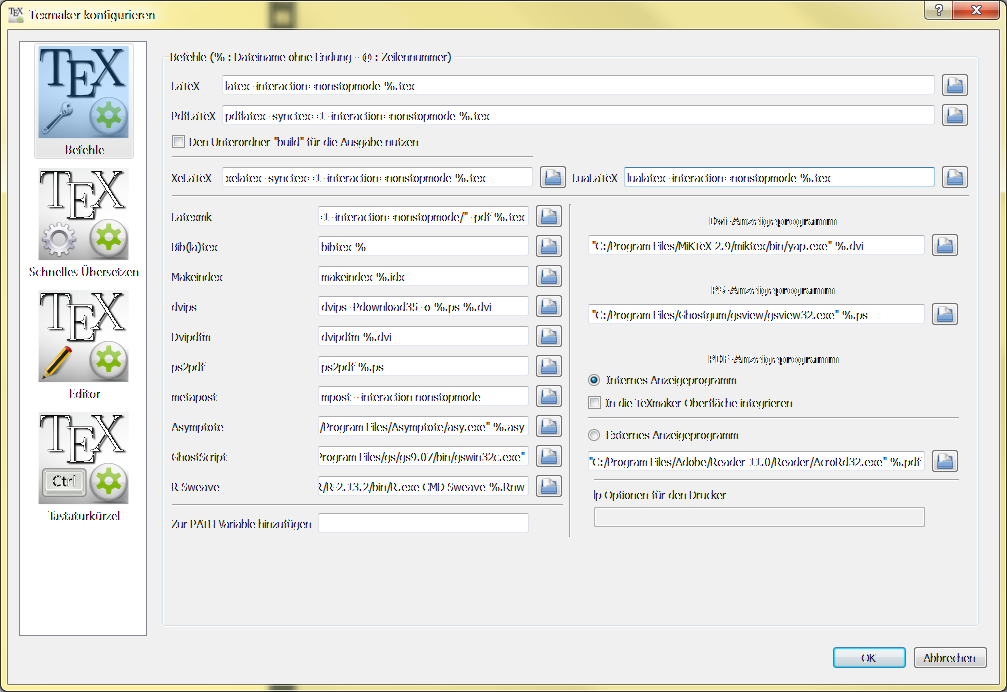
\includegraphics[width=\textwidth]{Bilder/Texmaker_konfigurieren.png} 
\caption{Dialog zum einrichten von Texmaker (hier Version 4.2)}
\label{img:texmaker_conf}
\end{figure}

Abbildung \ref{img:texmaker_conf} zeigt den Dialog zum Einrichten von Texmaker. Dieser ist über den Menüeintrag \verb+Optionen > Texmaker konfigurieren+ zu erreichen. Beim ersten Start stehen hier noch die Befehle ohne Pfadangabe. Ist MiKTex, oder texlive auf dem eigenen PC installiert, dann muss hier nichts mehr geändert werden. Anders sieht es an einem PC in der Uni aus. texlive ist auf einem zentralen Netzlaufwerk installiert, das eigene Betriebssystem weiß jedoch nichts davon. Man könnte jetzt dem Betriebssystem texlive über die Umgebungsvariable PATH bekannt machen, aber ich möchte einen anderen Weg vorführen. Dazu ruft man \verb+Optionen > Texmaker konfigurieren+ auf und es wird der in Abbildung \ref{img:texmaker_conf} zu sehende Dialog angezeigt. Bei allen benötigten \LaTeX-Befehlen (das sind eigentlich nur PdfLaTeX und Bib(la)tex) muss der Pfad angepasst werden. Dazu fügt man am Anfang des entsprechenden Textfeldes \verb+\\wwuappl2\W\TeX\texlive2010\bin\win32+ ein. Aus 

\begin{verbatim}
   pdflatex -synctex=1 -interaction=nonstopmode %.tex
\end{verbatim}

wird dadurch

\begin{verbatim}
   \\wwuappl2\W\TeX\texlive2010\bin\win32\pdflatex -synctex=1
      -interaction=nonstopmode %.tex
\end{verbatim}

\subsubsection{Schnelles Übersetzen einrichten}

\begin{figure}[bh]
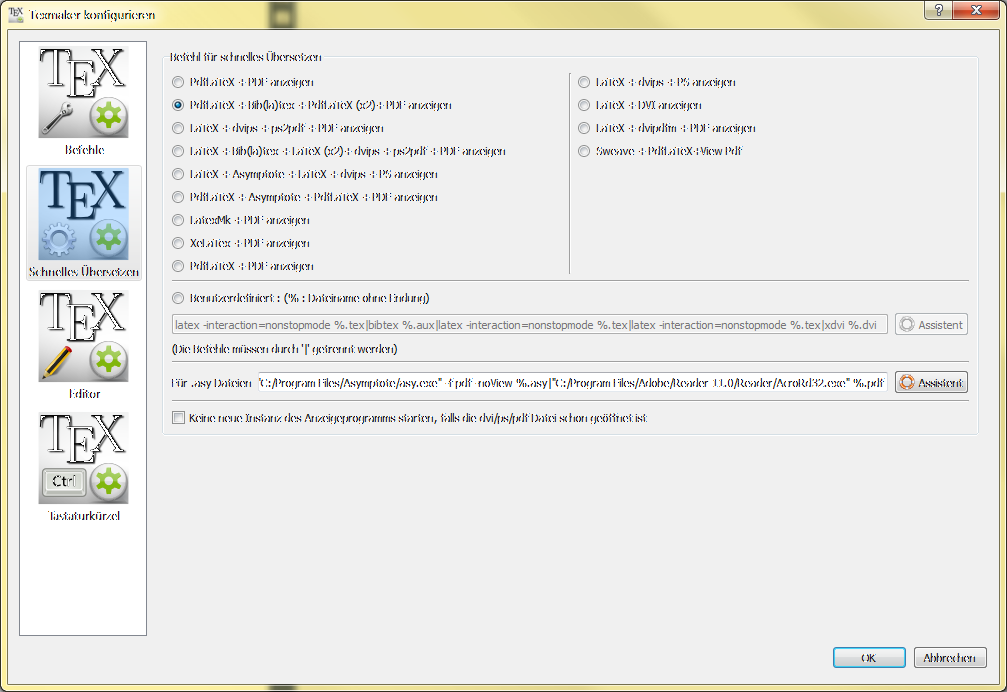
\includegraphics[width=\textwidth]{Bilder/Texmaker_konfigurieren2.png} 
\caption{Dialog zum einrichten von Texmaker (hier Version 4.2)}
\label{texmaker_konf2}
\end{figure}

Ruft man Schnelles Übersetzen auf (z.\,B. über die Toolbar, oder mit der Taste [F1]), dann wird PdfLaTeX einmal ausgeführt und anschließend die erzeugte PDF-Datei in Texmaler angezeigt. Hat sich das Inhaltsverzeichnis seid dem letzten Aufruf von PdfLaTeX verändert, oder sind neue Verweise eingefügt worden, dann fehlen diese Änderungen in der PDF-Datei. Deshalb ist es sinnvoll von  PdfLaTeX + PDF anzeigen auf PdfLaTeX + Bib(La)TeX + PdfLaTeX (2x) + PDF anzeigen umzustellen. Dazu ruft man \verb+Optionen > Texmaker konfigurieren+ auf und selektiert auf der linken Seite Schnelles Übersetzen (siehe Abblidung \ref{texmaker_konf2}). Dort kann man neben den genannten Optionen noch viele weitere auswählen.
	} % Nach \IfFileExists muss eine Leerzeile eingefügt werden

% ###################################
% # Literaturverzeichnis mit BibTeX #
% ###################################

	\setboolean{show}{\varZeigeLiteraturverzeichnis}
	\ifthenelse{\boolean{show}}{
	    \newpage
	    \bibliography{literatur}
	    \bibliographystyle{\varLiteraturLayout}
	}{}

% #######################
% # Ende des Dokumentes #
% #######################

\end{document}
